% ============================================================
%  Algebraic Reasoning Distiller  —  Flux Beamer  v3
%  Fondo claro, banners oscuros, fuente pequeña, espaciado generoso
% ============================================================
\documentclass[aspectratio=169,10pt]{beamer}

\usepackage[utf8]{inputenc}
\usepackage[T1]{fontenc}
\usepackage{amsmath,amssymb,amsfonts}
\usepackage{graphicx}
\usepackage{booktabs}
\usepackage{colortbl}
\usepackage{array}
\usepackage{xcolor}
\usepackage{tikz}
\usetikzlibrary{positioning,arrows.meta,fit,backgrounds,calc}

% ── Palette ─────────────────────────────────────────────────
\definecolor{SlideBackground}{HTML}{F4F6FB}   % almost-white
\definecolor{BannerDark}{HTML}{0D1117}         % near-black
\definecolor{BannerMid}{HTML}{1C2333}
\definecolor{AccentBlue}{HTML}{1E6FBF}
\definecolor{AccentCyan}{HTML}{0892C8}
\definecolor{AccentGreen}{HTML}{1A8C58}
\definecolor{AccentRed}{HTML}{C0392B}
\definecolor{AccentGold}{HTML}{B07D10}
\definecolor{AccentPurple}{HTML}{6A3E9E}
\definecolor{TextDark}{HTML}{1A1A2A}
\definecolor{TextMid}{HTML}{3A3A4A}
\definecolor{TextLight}{HTML}{F0F4FF}
\definecolor{BoxBg}{HTML}{E8EDF8}
\definecolor{BoxBgAlt}{HTML}{EAF5EA}

% ── Beamer colours ──────────────────────────────────────────
\setbeamercolor{background canvas}{bg=SlideBackground}
\setbeamercolor{normal text}{fg=TextDark}
\setbeamercolor{footline}{bg=BannerMid, fg=TextLight}
\setbeamercolor{frametitle}{fg=TextLight, bg=BannerDark}
\setbeamercolor{framesubtitle}{fg=AccentCyan}
\setbeamercolor{title}{fg=TextLight}
\setbeamercolor{structure}{fg=AccentBlue}
\setbeamercolor{itemize item}{fg=AccentBlue}
\setbeamercolor{itemize subitem}{fg=AccentCyan}
\setbeamercolor{block title}{bg=AccentBlue, fg=white}
\setbeamercolor{block body}{bg=BoxBg, fg=TextDark}
\setbeamercolor{alerted text}{fg=AccentRed}

% ── Fonts & sizes ───────────────────────────────────────────
\setbeamerfont{frametitle}{size=\small, series=\bfseries}
\setbeamerfont{framesubtitle}{size=\footnotesize}
\setbeamerfont{normal text}{size=\footnotesize}
\setbeamerfont{itemize/enumerate body}{size=\footnotesize}
\setbeamerfont{block title}{size=\footnotesize, series=\bfseries}
\setbeamerfont{block body}{size=\scriptsize}

% ── Templates ───────────────────────────────────────────────
\setbeamertemplate{navigation symbols}{}
\setbeamertemplate{itemize item}{\scriptsize$\blacktriangleright$}
\setbeamertemplate{itemize subitem}{\scriptsize$\triangleright$}

\setbeamertemplate{frametitle}{%
  \vskip0pt
  \begin{beamercolorbox}[wd=\paperwidth,ht=8mm,dp=2mm,leftskip=5mm]{frametitle}%
    \vbox to 8mm{\vfil
        \hbox{\usebeamerfont{frametitle}\insertframetitle
          \ifx\insertframesubtitle\@empty\else
            \hspace{3mm}\textcolor{AccentCyan}{\normalfont\footnotesize|}\hspace{3mm}%
            \textcolor{AccentCyan}{\usebeamerfont{framesubtitle}\insertframesubtitle}%
          \fi}%
        \vfil}%
  \end{beamercolorbox}%
}

\setbeamertemplate{footline}{%
  \begin{beamercolorbox}[wd=\paperwidth,ht=5mm,dp=1.5mm]{footline}%
    \vbox to 5mm{\vfil
        \hbox to \paperwidth{%
          \hspace{4mm}%
          \textcolor{TextLight}{\tiny Algebraic Reasoning Distiller}%
          \hfill
          \textcolor{TextLight}{\tiny SAIR — Mathematics Distillation Challenge}%
          \hfill
          \textcolor{AccentCyan}{\tiny\insertframenumber/\inserttotalframenumber}%
          \hspace{4mm}}%
        \vfil}%
  \end{beamercolorbox}%
}

% ── Helpers ─────────────────────────────────────────────────
\newcommand{\hl}[1]{\textcolor{AccentRed}{\textbf{#1}}}
\newcommand{\cy}[1]{\textcolor{AccentBlue}{\textbf{#1}}}
\newcommand{\gn}[1]{\textcolor{AccentGreen}{\textbf{#1}}}
\newcommand{\gd}[1]{\textcolor{AccentGold}{\textbf{#1}}}

% content area margin helper
\newcommand{\slidepad}{\vspace{3mm}\hspace{2mm}}

% ── TikZ node styles ────────────────────────────────────────
\tikzset{
  ND/.style={draw=#1, fill=#1!10, rounded corners=3pt,
      inner sep=5pt, align=center, text=TextDark, font=\scriptsize},
  ARR/.style={-Stealth, thick, #1},
}

% ============================================================
\begin{document}
\fontsize{9.5pt}{11.5pt}\selectfont
\footnotesize   % global default

% ============================================================
% SLIDE 1  ·  TITLE
% ============================================================
{
  \setbeamertemplate{footline}{}
  \begin{frame}[plain]

    \begin{tikzpicture}[remember picture,overlay]
      % Full dark background
      \fill[BannerDark] (current page.north west) rectangle (current page.south east);
      % Cyan accent strip left
      \fill[AccentBlue] (current page.north west) rectangle
      ([xshift=8mm]current page.south west);
      % Top gradient panel
      \fill[BannerMid] (current page.north west) rectangle
      ([yshift=-45mm]current page.north east);
      % Decorative triangles
      \begin{scope}[opacity=0.06]
        \fill[AccentCyan]
        ([xshift=0.55\paperwidth]current page.north west) --
        ([xshift=\paperwidth]current page.north west) --
        ([xshift=\paperwidth,yshift=-45mm]current page.north west) -- cycle;
      \end{scope}
      % Main title
      \node[anchor=west, xshift=14mm, yshift=14mm] at (current page.west){%
        \parbox{0.66\paperwidth}{%
          \textcolor{white}{\large\bfseries Algebraic Reasoning Distiller}\\[5pt]
          \textcolor{AccentCyan}{\normalsize
            Aprovechando la colaboración multiagente\\
            para la resolución de problemas matemáticos}\\[8pt]
          \textcolor{gray}{\scriptsize
            SAIR Foundation — Mathematics Distillation Challenge, Fase 1: Teorías ecuacionales}
        }};
      % Authors
      \node[anchor=south west, xshift=14mm, yshift=12mm]
      at (current page.south west){%
        \parbox{0.85\paperwidth}{%
          \textcolor{white}{\scriptsize
            Joaquín Mir Macías $\cdot$
            Miguel Montes Lorenzo $\cdot$
            José Andrés Ridruejo Tuñón $\cdot$
            Javier Ríos Montes
          }\\[2pt]
          \textcolor{gray}{\tiny
            Deep Generative Models $\cdot$ Máster en Inteligencia Artificial $\cdot$
            U.P.Comillas 2026}}};
    \end{tikzpicture}
  \end{frame}
}

% ============================================================
% SLIDE 2  ·  MOTIVATION VISUAL
% ============================================================
\begin{frame}{Motivación}{Contexto del reto}
  \vspace{2mm}
  \centering

  \begin{columns}[T,onlytextwidth]
    \begin{column}{0.38\textwidth}
      \centering
      \begin{minipage}[b][0.62\textheight][c]{\linewidth}
        \centering
        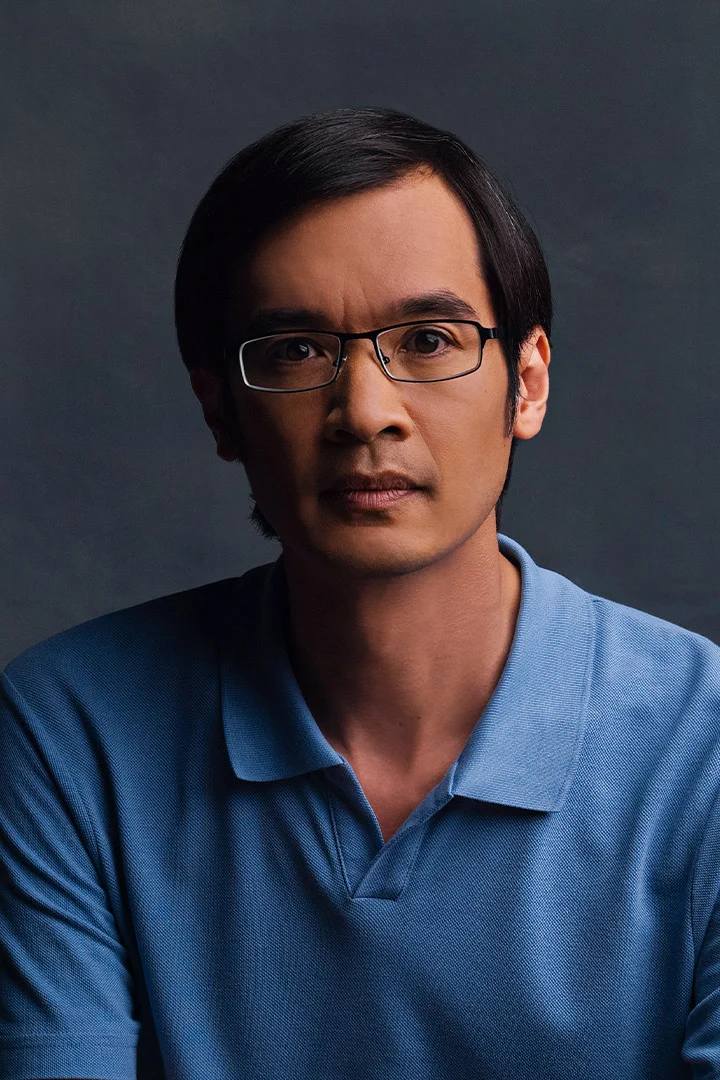
\includegraphics[height=0.62\textheight,keepaspectratio]{figures/tao.png}
      \end{minipage}

      \vspace{2mm}
      \parbox{0.92\linewidth}{\centering\scriptsize
        Terence Tao, asociado con la SAIR Foundation y con la
        motivación más amplia detrás del razonamiento matemático formal.
      }
    \end{column}
    \hfill
    \begin{column}{0.58\textwidth}
      \centering
      \begin{minipage}[b][0.62\textheight][c]{\linewidth}
        \centering
        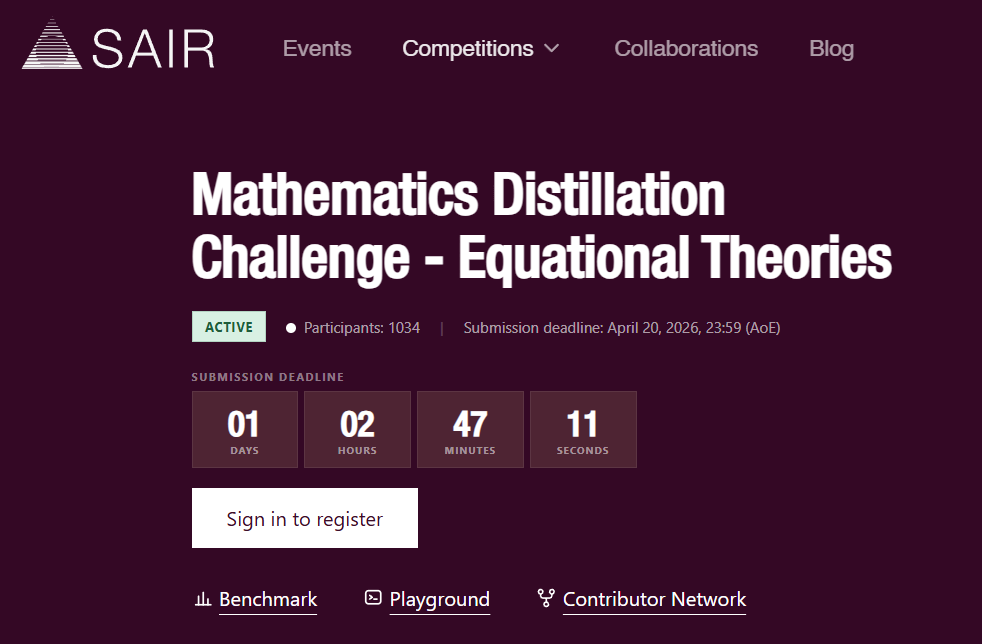
\includegraphics[height=0.62\textheight,keepaspectratio]{figures/sair-landing.png}
      \end{minipage}

      \vspace{2mm}
      \parbox{0.95\linewidth}{\centering\scriptsize
        Página principal del SAIR Mathematics Distillation Challenge:
        \textit{Equational Theories}.
      }
    \end{column}
  \end{columns}

\end{frame}

% ============================================================
% SLIDE 2  ·  MOTIVATION
% ============================================================
\begin{frame}{Motivación}{¿Por qué sigue fallando el razonamiento matemático?}
  \begin{center}
    \begin{minipage}{0.72\textwidth}
      \vspace{2mm}

      \hspace*{\leftmargini}\cy{La brecha en el razonamiento matemático de los LLM:}

      \vspace{2mm}
      \begin{itemize}\setlength\itemsep{4pt}
        \item Los LLM resuelven matemáticas mediante \hl{pattern matching}, no mediante comprensión simbólica
        \item Errores sistemáticos en manipulación algebraica e inferencia abstracta
        \item El \textbf{pretraining} sobre corpus matemáticos es prohibitivamente costoso
        \item Un \textbf{fine-tuning} ingenuo produce expertos demasiado estrechos
        \item Incluso los modelos más avanzados muestran debilidades en álgebra abstracta
      \end{itemize}

      \vspace{3mm}
      \begin{block}{Nuestro enfoque}
        \textbf{Razonamiento simbólico} + \textbf{destilación de LLM} mediante
        cómputo multiagente offline, dentro de restricciones estrictas de competición.
      \end{block}
    \end{minipage}
  \end{center}
\end{frame}

% ============================================================
% SLIDE 3  ·  PROBLEM STATEMENT
% ============================================================
\begin{frame}{El reto}{SAIR. Mathematics Distillation Challenge}
  \begin{columns}[T,onlytextwidth]
    \begin{column}{0.50\textwidth}
      \vspace{4mm}
      \cy{Formulación matemática:}
      \vspace{3mm}

      Un \textbf{magma} es un conjunto $M$ con una operación binaria
      ${\ast}:M\!\times\!M\to M$ \textit{(sin asumir axiomas)}.

      \vspace{4mm}
      Dados $E_1, E_2$ construidos con $\ast$, decidir:
      \[
        \boxed{\;E_1 \;\overset{?}{\Longrightarrow}\; E_2
          \;\text{ en todo magma}\;}
      \]

      \vspace{4mm}
      \textbf{Ejemplo:}\\[3pt]
      $E_1{:}\; x \ast y = z \ast (w \ast (u \ast u))$\\[2pt]
      $E_2{:}\; x \ast (y \ast y) = (z \ast w) \ast z$\\[4pt]
      \gn{Respuesta: TRUE}
      \hfill\textcolor{gray}{\tiny todo magma que satisface $E_1$ también satisface $E_2$}
    \end{column}
    \hfill
    \begin{column}{0.46\textwidth}
      \vspace{2mm}
      \cy{Restricciones de la competición:}
      \vspace{2mm}

      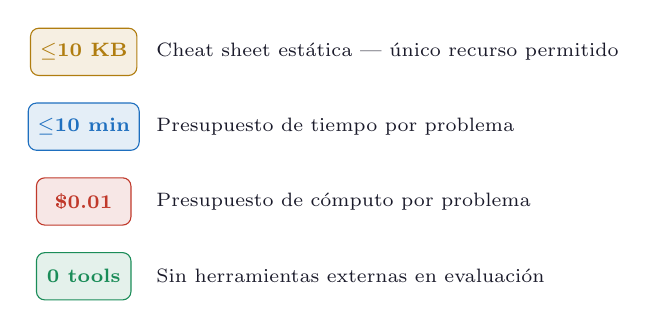
\begin{tikzpicture}[every node/.style={font=\scriptsize}]
        \foreach \y/\col/\badge/\desc in {
        0.0/AccentGold/{$\leq$10 KB}/{Cheat sheet estática — único recurso permitido},
        -0.95/AccentBlue/{$\leq$10 min}/{Presupuesto de tiempo por problema},
        -1.90/AccentRed/{\$0.01}/{Presupuesto de cómputo por problema},
        -2.85/AccentGreen/{0 tools}/{Sin herramientas externas en evaluación}
        }{
        \node[draw=\col, fill=\col!12, rounded corners=3pt,
          minimum width=1.2cm, minimum height=6mm,
          font=\bfseries\scriptsize, text=\col, align=center]
        at (0,\y) {\badge};
        \node[anchor=west, text=TextDark] at (0.8,\y) {\desc};
        }
      \end{tikzpicture}

      \vspace{4mm}
      \begin{block}{Idea clave}
        Todo el cómputo pesado ocurre \textbf{offline}.
        En test: cheat sheet + una llamada al LLM.
      \end{block}
    \end{column}
  \end{columns}
\end{frame}

% ============================================================
% SLIDE 4  ·  SYSTEM ARCHITECTURE
% ============================================================
\begin{frame}{Arquitectura del sistema}{Algebraic Reasoning Distiller (ARD)}
  \vspace{1mm}
  \centering
  \resizebox{0.96\textwidth}{!}{%
    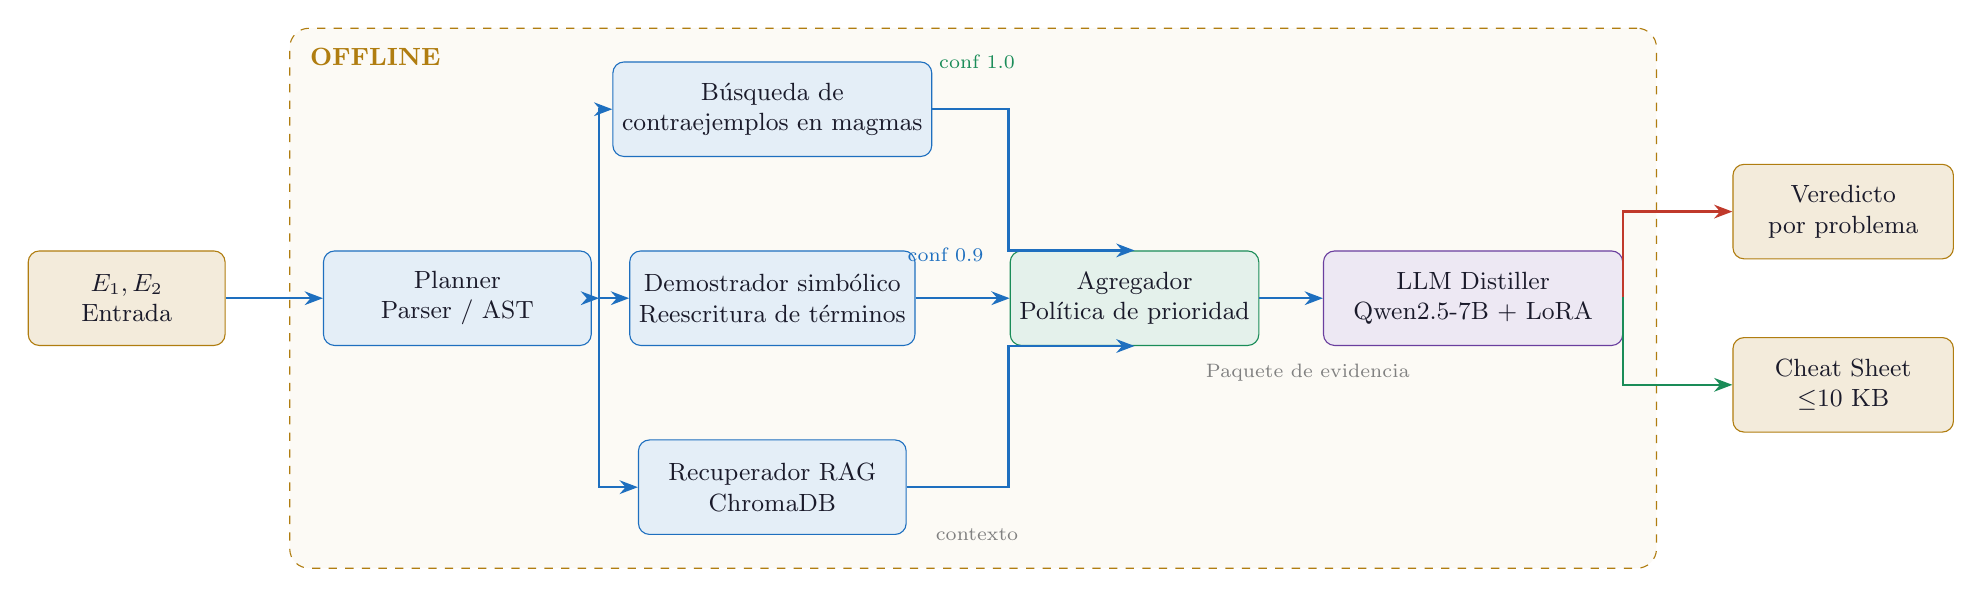
\begin{tikzpicture}[
        every node/.style={font=\small},
        IN/.style={draw=AccentGold,   fill=AccentGold!15,   rounded corners=4pt,
            minimum height=12mm, minimum width=25mm,
            align=center, text=TextDark},
        OT/.style={draw=AccentGold,   fill=AccentGold!15,   rounded corners=4pt,
            minimum height=12mm, minimum width=28mm,
            align=center, text=TextDark},
        AG/.style={draw=AccentBlue,   fill=AccentBlue!12,   rounded corners=4pt,
            minimum height=12mm, minimum width=34mm,
            align=center, text=TextDark},
        GR/.style={draw=AccentGreen,  fill=AccentGreen!12,  rounded corners=4pt,
            minimum height=12mm, minimum width=31mm,
            align=center, text=TextDark},
        LM/.style={draw=AccentPurple, fill=AccentPurple!12, rounded corners=4pt,
            minimum height=12mm, minimum width=38mm,
            align=center, text=TextDark},
        arr/.style={-Stealth, thick, AccentBlue},
        darr/.style={-Stealth, thick, AccentRed},
        garr/.style={-Stealth, thick, AccentGreen},
      ]

      % Main nodes
      \node[IN] (inp)  at (-1.0, 0.0) {$E_1,E_2$\\Entrada};
      \node[AG] (plan) at (3.2, 0.0) {Planner\\Parser / AST};

      \node[AG] (cex)  at (7.2, 2.4) {Búsqueda de\\contraejemplos en magmas};
      \node[AG] (sym)  at (7.2, 0.0) {Demostrador simbólico\\Reescritura de términos};
      \node[AG] (rag)  at (7.2,-2.4) {Recuperador RAG\\ChromaDB};

      \node[GR] (agg)  at (11.8, 0.0) {Agregador\\Política de prioridad};
      \node[LM] (llm)  at (16.1, 0.0) {LLM Distiller\\Qwen2.5-7B + LoRA};

      \node[OT] (verd) at (20.8, 1.1) {Veredicto\\por problema};
      \node[OT] (cs)   at (20.8,-1.1) {Cheat Sheet\\$\leq$10 KB};

      % Branch helper coordinates
      \coordinate (fork1) at (5.0, 0.0);
      \coordinate (joinTop) at (10.2, 2.4);
      \coordinate (joinBot) at (10.2,-2.4);
      \coordinate (outSplit) at (18.0, 0.0);

      % Arrows
      \draw[arr] (inp.east) -- (plan.west);
      \draw[arr] (plan.east) -- (fork1);
      \draw[arr] (fork1) |- (cex.west);
      \draw[arr] (fork1) -- (sym.west);
      \draw[arr] (fork1) |- (rag.west);

      \draw[arr] (cex.east) -- (joinTop) |- (agg.north);
      \draw[arr] (sym.east) -- (agg.west);
      \draw[arr] (rag.east) -- (joinBot) |- (agg.south);

      \draw[arr] (agg.east) -- (llm.west);
      \draw[darr] (llm.east) -- (outSplit) |- (verd.west);
      \draw[garr] (llm.east) -- (outSplit) |- (cs.west);

      % Labels
      \node[font=\scriptsize, text=AccentGreen] at (9.8, 3.0) {conf 1.0};
      \node[font=\scriptsize, text=AccentBlue]  at (9.4, 0.55) {conf 0.9};
      \node[font=\scriptsize, text=gray]        at (9.8,-3.0) {contexto};
      \node[font=\scriptsize, text=gray]        at (14.0,-0.95) {Paquete de evidencia};

      % Offline box
      \begin{scope}[on background layer]
        \node[draw=AccentGold, dashed, fill=AccentGold!4,
          rounded corners=7pt,
          fit=(plan)(cex)(sym)(rag)(agg)(llm),
          inner sep=12pt] (offbox) {};
      \end{scope}

      \node[font=\small\bfseries, text=AccentGold,
        anchor=north west, xshift=4pt, yshift=-4pt]
      at (offbox.north west) {OFFLINE};

    \end{tikzpicture}%
  }
\end{frame}

% ============================================================
% SLIDE 5  ·  PLANNER
% ============================================================
\begin{frame}{Agente: Planner}{Parseo de ecuaciones a árboles de sintaxis abstracta}
  \begin{columns}[T,onlytextwidth]
    \begin{column}{0.46\textwidth}
      \vspace{4mm}
      \cy{Parser recursivo descendente}\\[5pt]
      Cadena de entrada $\to$ AST como tupla anidada:

      \vspace{6mm}
      \centering
      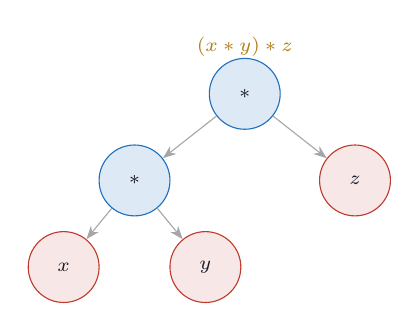
\begin{tikzpicture}[
          nd/.style={circle, draw=AccentBlue, fill=AccentBlue!15,
              text=TextDark, font=\scriptsize,
              inner sep=0pt, minimum size=9mm},
          lf/.style={circle, draw=AccentRed, fill=AccentRed!12,
              text=TextDark, font=\scriptsize,
              inner sep=0pt, minimum size=9mm},
          ar/.style={-Stealth, gray!70, thin},
        ]
        \node[font=\scriptsize, text=AccentGold] at (0, 0.6) {$(x \ast y)\ast z$};
        \node[nd] (r)  at (0,  0)   {$\ast$};
        \node[nd] (l)  at (-1.4,-1.1) {$\ast$};
        \node[lf] (rr) at ( 1.4,-1.1) {$z$};
        \node[lf] (ll) at (-2.3,-2.2) {$x$};
        \node[lf] (lr) at (-0.5,-2.2) {$y$};
        \draw[ar] (r)--(l); \draw[ar] (r)--(rr);
        \draw[ar] (l)--(ll); \draw[ar] (l)--(lr);
      \end{tikzpicture}

      \vspace{4mm}
      \centering\texttt{\scriptsize ("mul", ("mul", ("var","x"), ("var","y")), ("var","z"))}
    \end{column}
    \hfill
    \begin{column}{0.50\textwidth}
      \vspace{4mm}
      \cy{¿Por qué AST?}
      \vspace{3mm}
      \begin{itemize}\setlength\itemsep{6pt}
        \item Representación canónica \textbf{compartida por todos los agentes}
        \item Permite comparación estructural:\\
              alfa-equivalencia, sustitución
        \item Desacopla la \textbf{sintaxis superficial} del contenido matemático
        \item Variables: \texttt{("var","x")}\\
              Operaciones: \texttt{("mul", left, right)}
      \end{itemize}
      \vspace{6mm}
      \begin{block}{Principio de diseño}
        Cada agente recibe el mismo AST ---
        los errores se propagan limpiamente y la pipeline
        \textbf{nunca falla} ante entradas mal formadas.
      \end{block}
    \end{column}
  \end{columns}
\end{frame}

% ============================================================
% SLIDE 6  ·  COUNTEREXAMPLE + SYMBOLIC
% ============================================================
\begin{frame}{Agentes: Counterexample \& Symbolic Prover}{Recogida de evidencia fuerte}
  \begin{columns}[T,onlytextwidth]
    \begin{column}{0.48\textwidth}
      \vspace{4mm}
      \cy{Generador de contraejemplos}\\[4pt]
      \scriptsize Buscar un magma $M$ tal que: $E_1$ se cumpla y $E_2$ falle.

      \vspace{5mm}
      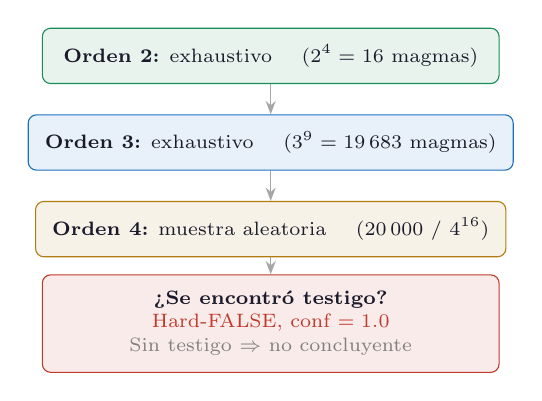
\begin{tikzpicture}[every node/.style={font=\scriptsize},
          ar/.style={-Stealth,gray!70,thin}]
        \node[draw=AccentGreen, fill=AccentGreen!10, rounded corners=3pt,
          minimum width=5.8cm, inner sep=6pt, align=left, text=TextDark]
        (o2) at (0,0)
        {\textbf{Orden 2:} exhaustivo \quad ($2^4=16$ magmas)};
        \node[draw=AccentBlue, fill=AccentBlue!10, rounded corners=3pt,
          minimum width=5.8cm, inner sep=6pt, align=left, text=TextDark]
        (o3) at (0,-1.1)
        {\textbf{Orden 3:} exhaustivo \quad ($3^9=19\,683$ magmas)};
        \node[draw=AccentGold, fill=AccentGold!10, rounded corners=3pt,
          minimum width=5.8cm, inner sep=6pt, align=left, text=TextDark]
        (o4) at (0,-2.2)
        {\textbf{Orden 4:} muestra aleatoria \quad (20\,000 / $4^{16}$)};
        \node[draw=AccentRed, fill=AccentRed!10, rounded corners=3pt,
          minimum width=5.8cm, inner sep=6pt, align=center, text=TextDark]
        (res) at (0,-3.4)
        {\textbf{¿Se encontró testigo?}\\
          \textcolor{AccentRed}{Hard-FALSE, conf $= 1.0$}\\[1pt]
          \textcolor{gray}{Sin testigo $\Rightarrow$ no concluyente}};
        \draw[ar](o2)--(o3); \draw[ar](o3)--(o4); \draw[ar](o4)--(res);
      \end{tikzpicture}
    \end{column}
    \hfill
    \begin{column}{0.48\textwidth}
      \vspace{4mm}
      \cy{Demostrador simbólico}\\[4pt]
      \scriptsize Tres estrategias, aplicadas en orden:

      \vspace{5mm}
      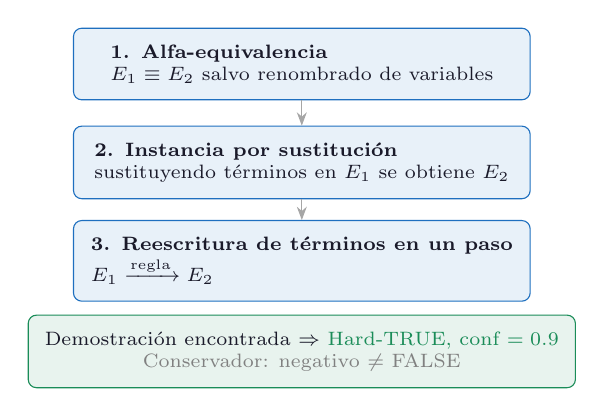
\begin{tikzpicture}[every node/.style={font=\scriptsize},
          ar/.style={-Stealth,gray!70,thin}]
        \node[draw=AccentBlue, fill=AccentBlue!10, rounded corners=3pt,
          minimum width=5.8cm, inner sep=6pt, align=left, text=TextDark]
        (a1) at (0,0)
        {\textbf{1. Alfa-equivalencia}\\
          $E_1 \equiv E_2$ salvo renombrado de variables};
        \node[draw=AccentBlue, fill=AccentBlue!10, rounded corners=3pt,
          minimum width=5.8cm, inner sep=6pt, align=left, text=TextDark]
        (a2) at (0,-1.25)
        {\textbf{2. Instancia por sustitución}\\
          sustituyendo términos en $E_1$ se obtiene $E_2$};
        \node[draw=AccentBlue, fill=AccentBlue!10, rounded corners=3pt,
          minimum width=5.8cm, inner sep=6pt, align=left, text=TextDark]
        (a3) at (0,-2.5)
        {\textbf{3. Reescritura de términos en un paso}\\
          $E_1 \xrightarrow{\text{regla}} E_2$};
        \node[draw=AccentGreen, fill=AccentGreen!10, rounded corners=3pt,
          minimum width=5.8cm, inner sep=6pt, align=center, text=TextDark]
        at (0,-3.65)
        {Demostración encontrada $\Rightarrow$
          \textcolor{AccentGreen}{Hard-TRUE, conf $= 0.9$}\\
          \textcolor{gray}{Conservador: negativo $\neq$ FALSE}};
        \draw[ar](a1)--(a2); \draw[ar](a2)--(a3);
      \end{tikzpicture}
    \end{column}
  \end{columns}
\end{frame}

% ============================================================
% SLIDE 7  ·  RAG + AGGREGATOR
% ============================================================
\begin{frame}{Agentes: RAG Retriever \& Aggregator}{Inyección de contexto y política de prioridad}
  \begin{columns}[T,onlytextwidth]
    \begin{column}{0.44\textwidth}
      \vspace{4mm}
      \cy{RAG Retriever}
      \vspace{5mm}

      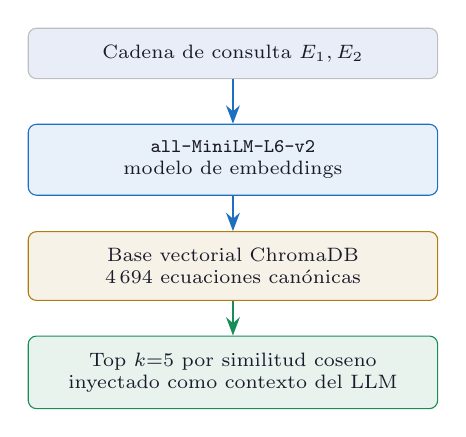
\begin{tikzpicture}[every node/.style={font=\scriptsize},
          ar/.style={-Stealth,thick,AccentBlue}]
        \node[draw=gray!50,    fill=BoxBg,           rounded corners=3pt,
          minimum width=5.2cm, inner sep=6pt, align=center, text=TextDark]
        (q)  at (0, 0.0)   {Cadena de consulta $E_1, E_2$};
        \node[draw=AccentBlue, fill=AccentBlue!10,  rounded corners=3pt,
          minimum width=5.2cm, inner sep=6pt, align=center, text=TextDark]
        (em) at (0,-1.35) {\texttt{all-MiniLM-L6-v2}\\modelo de embeddings};
        \node[draw=AccentGold, fill=AccentGold!10,  rounded corners=3pt,
          minimum width=5.2cm, inner sep=6pt, align=center, text=TextDark]
        (db) at (0,-2.70) {Base vectorial ChromaDB\\4\,694 ecuaciones canónicas};
        \node[draw=AccentGreen,fill=AccentGreen!10, rounded corners=3pt,
          minimum width=5.2cm, inner sep=6pt, align=center, text=TextDark]
        (out)at (0,-4.05) {Top $k{=}5$ por similitud coseno\\inyectado como contexto del LLM};

        \draw[ar] (q.south) -- (em.north);
        \draw[ar] (em.south) -- (db.north);
        \draw[-Stealth,thick,AccentGreen] (db.south) -- (out.north);
      \end{tikzpicture}
      \vspace{3pt}
      \textcolor{gray}{\tiny Degrada de forma estable si el índice no está disponible.}
    \end{column}
    \hfill
    \begin{column}{0.52\textwidth}
      \vspace{4mm}
      \cy{Aggregator (por orden de prioridades prioridad)}
      \vspace{5mm}

      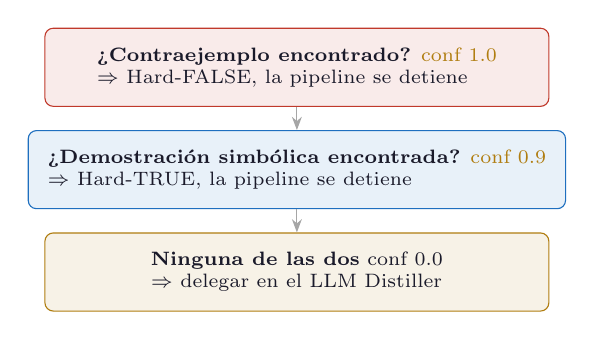
\begin{tikzpicture}[every node/.style={font=\scriptsize},
          ar/.style={-Stealth,gray!70,thin}]
        \node[draw=AccentRed,   fill=AccentRed!10,   rounded corners=3pt,
          minimum width=6.4cm, inner sep=7pt, align=left, text=TextDark]
        (c1) at (0, 0)
        {\textbf{¿Contraejemplo encontrado?}
          \hfill\textcolor{AccentGold}{conf 1.0}\\
          $\Rightarrow$ Hard-FALSE, la pipeline se detiene};
        \node[draw=AccentBlue,  fill=AccentBlue!10,  rounded corners=3pt,
          minimum width=6.4cm, inner sep=7pt, align=left, text=TextDark]
        (c2) at (0,-1.3)
        {\textbf{¿Demostración simbólica encontrada?}
          \hfill\textcolor{AccentGold}{conf 0.9}\\
          $\Rightarrow$ Hard-TRUE, la pipeline se detiene};
        \node[draw=AccentGold,  fill=AccentGold!10,  rounded corners=3pt,
          minimum width=6.4cm, inner sep=7pt, align=left, text=TextDark]
        (c3) at (0,-2.6)
        {\textbf{Ninguna de las dos} \hfill conf 0.0\\
          $\Rightarrow$ delegar en el LLM Distiller};
        \draw[ar](c1)--(c2); \draw[ar](c2)--(c3);
      \end{tikzpicture}
      \vspace{2mm}
      \textcolor{gray}{\scriptsize Resultado negativo $\neq$ falsedad: el demostrador es deliberadamente conservador.}
    \end{column}
  \end{columns}
\end{frame}

% ============================================================
% SLIDE 8  ·  LLM DISTILLER
% ============================================================
\begin{frame}{Agente: LLM Distiller}{Qwen2.5-7B + LoRA. Arquitectura y modos de inferencia}
  \begin{columns}[T,onlytextwidth]
    \begin{column}{0.46\textwidth}
      \vspace{4mm}
      \cy{Pila del modelo:}
      \vspace{5mm}

      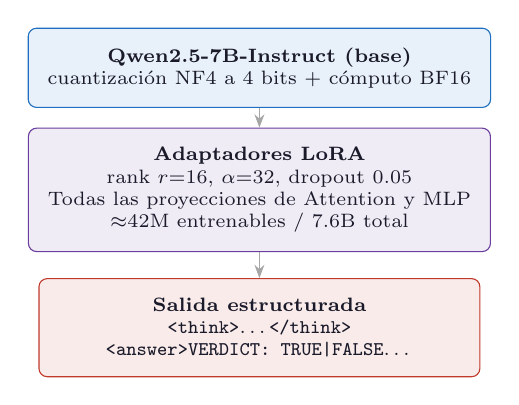
\begin{tikzpicture}[every node/.style={font=\scriptsize},
          ar/.style={-Stealth,gray!70,thin}]
        \node[draw=AccentBlue,  fill=AccentBlue!10,  rounded corners=3pt,
          minimum width=5.6cm, inner sep=7pt, align=center, text=TextDark]
        (base) at (0,0)
        {\textbf{Qwen2.5-7B-Instruct (base)}\\
          cuantización NF4 a 4 bits + cómputo BF16};
        \node[draw=AccentPurple,fill=AccentPurple!10,rounded corners=3pt,
          minimum width=5.6cm, inner sep=7pt, align=center, text=TextDark]
        (lora) at (0,-1.55)
        {\textbf{Adaptadores LoRA}\\
          rank $r{=}16$,\ $\alpha{=}32$,\ dropout $0.05$\\
          Todas las proyecciones de Attention y MLP\\
          $\approx$42M entrenables / 7.6B total};
        \node[draw=AccentRed,   fill=AccentRed!10,   rounded corners=3pt,
          minimum width=5.6cm, inner sep=7pt, align=center, text=TextDark]
        (out) at (0,-3.30)
        {\textbf{Salida estructurada}\\
          \texttt{<think>}\ldots\texttt{</think>}\\
          \texttt{<answer>VERDICT: TRUE|FALSE}\ldots};
        \draw[ar](base)--(lora); \draw[ar](lora)--(out);
      \end{tikzpicture}
    \end{column}
    \hfill
    \begin{column}{0.50\textwidth}
      \vspace{3mm}
      \cy{Dos modos de inferencia:}
      \vspace{4mm}

      \begin{block}{Modo por problema}
        \textbf{Entrada:} EvidenceBundle + contexto RAG\\
        \textbf{Salida:} chain-of-thought + VERDICT
      \end{block}

      \vspace{3mm}

      \begin{block}{Modo de síntesis de cheat sheet}
        \textbf{Entrada:} clúster de problemas similares\\
        \textbf{Salida:} bloque de lemas de $\leq$1\,200 bytes\\
        Los tokens \texttt{VERDICT} están \textbf{prohibidos} en el prompt de síntesis
      \end{block}

      \vspace{3mm}
      \cy{¿Por qué Qwen2.5-7B?}\\[3pt]
      \scriptsize
      Cabe en 4 bits en una sola GPU $\cdot$
      satisface el presupuesto de \$0.01/problema $\cdot$
      base matemática sólida
    \end{column}
  \end{columns}
\end{frame}

% ============================================================
% SLIDE 9  ·  DATASET
% ============================================================
\begin{frame}{Dataset}{Corpus de entrenamiento e índice de recuperación}
  \vspace{1mm}

  \centering
  \scalebox{0.8}{%
    \begin{minipage}{1.15\textwidth}

      \footnotesize
      \setlength\arrayrulewidth{0.3pt}
      \arrayrulecolor{gray!35}
      \renewcommand{\arraystretch}{1.12}

      \begin{tabular}{p{3.5cm}rp{5.7cm}}
        \toprule
        \rowcolor{BannerDark}
        \textcolor{white}{\textbf{Fuente}}                      &
        \textcolor{white}{\textbf{\#}}                          &
        \textcolor{white}{\textbf{Notas}}                                                                                                                   \\
        \midrule
        \rowcolor{BoxBg}
        SAIR judge repo                                         & 20     & ejemplos canónicos etiquetados                                                   \\
        Playground hard3                                        & 72     & conjunto playground curado manualmente                                           \\
        \rowcolor{BoxBg}
        Competition dumps                                       & 1\,669 & \texttt{hard.txt}, \texttt{hard2.txt}, \texttt{hard3.txt}, \texttt{normales.txt} \\
        Retrieval index (RAG)                                   & 4\,694 & ecuaciones embebidas en ChromaDB solo para recuperación                          \\
        \midrule
        \rowcolor{BannerDark}
        \textcolor{white}{\textbf{Total del corpus etiquetado}} &
        \textcolor{white}{\textbf{1\,761}}                      &
        \textcolor{white}{corpus de entrenamiento/evaluación}                                                                                               \\
        \bottomrule
      \end{tabular}

      \vspace{4mm}

      \begin{columns}[T,onlytextwidth]
        \begin{column}{0.37\textwidth}
          \textbf{Partición Train / Eval:}\\[3pt]
          \textcolor{AccentBlue}{\textbf{80\%}} train --- 1\,409 problemas\\[2pt]
          \textcolor{AccentRed}{\textbf{20\%}} eval \phantom{0}--- 352 problemas

          \vspace{4mm}
          \textbf{Filtrado para SFT:}\\[3pt]
          \textcolor{gray}{\scriptsize
            Los problemas en los que el veredicto de la pipeline $\neq$ ground truth
            se excluyen del SFT.\\
            Permanecen aproximadamente 1\,330 ejemplos limpios.}

          \vspace{4mm}
          \textcolor{gray}{\tiny
            El tamaño del índice RAG se informa por separado del corpus etiquetado.}
        \end{column}
        \hfill
        \begin{column}{0.59\textwidth}
          \centering
          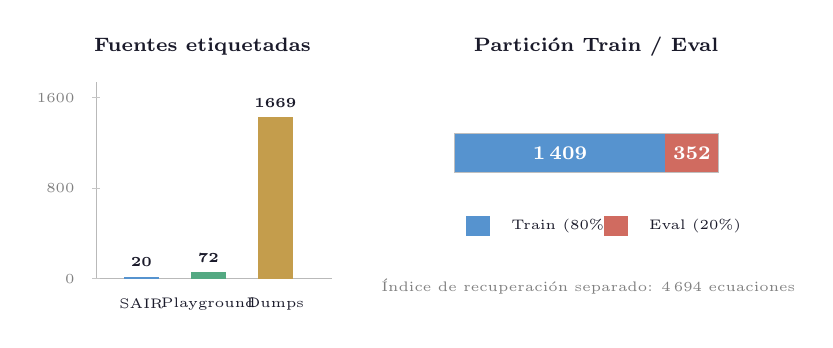
\begin{tikzpicture}[x=1cm,y=1cm]
            \node[font=\scriptsize\bfseries, text=TextDark] at (1.55,3.35)
            {Fuentes etiquetadas};

            \draw[gray!55, thin] (0.2,0.4) -- (0.2,2.9);
            \draw[gray!55, thin] (0.2,0.4) -- (3.2,0.4);

            \foreach \y/\lab in {0.4/0,1.55/800,2.7/1600} {
                \draw[gray!45, thin] (0.15,\y) -- (0.25,\y);
                \node[anchor=east, font=\tiny, text=gray] at (0.05,\y) {\lab};
              }

            \fill[AccentBlue!75]  (0.55,0.4) rectangle (1.00,0.43);
            \fill[AccentGreen!75] (1.40,0.4) rectangle (1.85,0.49);
            \fill[AccentGold!75]  (2.25,0.4) rectangle (2.70,2.45);

            \node[font=\tiny\bfseries, text=TextDark, anchor=south] at (0.775,0.43) {20};
            \node[font=\tiny\bfseries, text=TextDark, anchor=south] at (1.625,0.49) {72};
            \node[font=\tiny\bfseries, text=TextDark, anchor=south] at (2.475,2.45) {1669};

            \node[font=\tiny, align=center, text=TextDark] at (0.775,0.08) {SAIR};
            \node[font=\tiny, align=center, text=TextDark] at (1.625,0.08) {Playground};
            \node[font=\tiny, align=center, text=TextDark] at (2.475,0.08) {Dumps};

            \node[font=\scriptsize\bfseries, text=TextDark] at (6.55,3.35)
            {Partición Train / Eval};

            \fill[AccentBlue!75] (4.75,1.75) rectangle (7.43,2.25);
            \fill[AccentRed!75]  (7.43,1.75) rectangle (8.10,2.25);
            \draw[gray!50, thin] (4.75,1.75) rectangle (8.10,2.25);

            \node[font=\scriptsize\bfseries, text=white] at (6.09,2.00) {1\,409};
            \node[font=\scriptsize\bfseries, text=white] at (7.765,2.00) {352};

            \fill[AccentBlue!75] (4.90,0.95) rectangle (5.20,1.20);
            \node[anchor=west, font=\tiny, text=TextDark] at (5.35,1.075)
            {Train (80\%)};

            \fill[AccentRed!75] (6.65,0.95) rectangle (6.95,1.20);
            \node[anchor=west, font=\tiny, text=TextDark] at (7.10,1.075)
            {Eval (20\%)};

            \node[font=\tiny, text=gray, align=center] at (6.45,0.30)
            {Índice de recuperación separado: 4\,694 ecuaciones};
          \end{tikzpicture}
        \end{column}
      \end{columns}

    \end{minipage}%
  }
\end{frame}

% ============================================================
% SLIDE 10  ·  SFT
% ============================================================
\begin{frame}{Etapa de entrenamiento 1}{Supervised Fine-Tuning (SFT)}
  \begin{columns}[T,onlytextwidth]
    \begin{column}{0.50\textwidth}
      \vspace{4mm}
      \cy{EvidenceBundle $\to$ completion estructurada:}
      \vspace{4mm}

      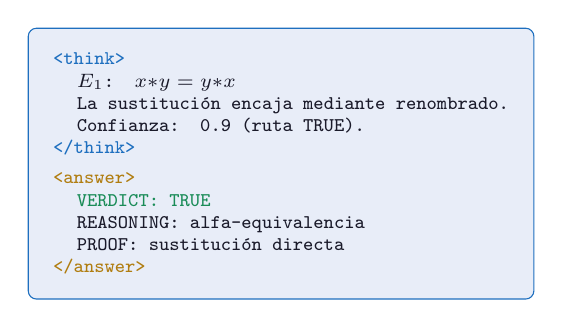
\begin{tikzpicture}
        \node[draw=AccentBlue, fill=BoxBg, rounded corners=3pt,
          minimum width=6.4cm, inner sep=9pt,
          align=left, text=TextDark, font=\ttfamily\scriptsize]{%
          \textcolor{AccentBlue}{<think>}\\
          \hspace{3mm}$E_1$: $x{*}y = y{*}x$\\
          \hspace{3mm}La sustitución encaja mediante renombrado.\\
          \hspace{3mm}Confianza: 0.9 (ruta TRUE).\\
          \textcolor{AccentBlue}{</think>}\\[3pt]
          \textcolor{AccentGold}{<answer>}\\
          \hspace{3mm}\textcolor{AccentGreen}{VERDICT: TRUE}\\
          \hspace{3mm}REASONING: alfa-equivalencia\\
          \hspace{3mm}PROOF: sustitución directa\\
          \textcolor{AccentGold}{</answer>}
        };
      \end{tikzpicture}
    \end{column}
    \hfill
    \begin{column}{0.46\textwidth}
      \vspace{4mm}
      \cy{Hiperparámetros:}
      \vspace{4mm}

      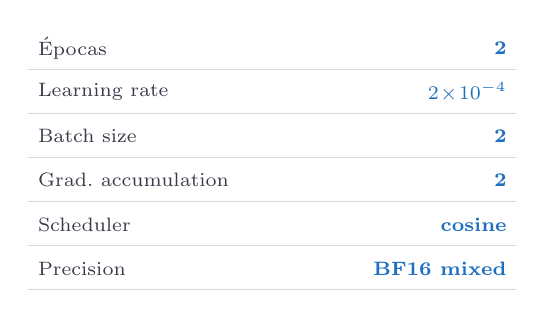
\begin{tikzpicture}[every node/.style={font=\scriptsize}]
        \foreach \k/\v/\i in {
        Épocas/2/0,
        {Learning rate}/$2\!\times\!10^{-4}$/1,
        {Batch size}/2/2,
        {Grad.\ accumulation}/2/3,
        Scheduler/cosine/4,
        Precision/{BF16 mixed}/5%
        }{
        \pgfmathsetmacro\yy{-\i * 0.56}
        \node[anchor=west, text=TextMid] at (0,\yy) {\k};
        \node[anchor=east, text=AccentBlue, font=\scriptsize\bfseries]
        at (6.2,\yy) {\v};
        \draw[gray!30, thin] (0,\yy-0.27) -- (6.2,\yy-0.27);
        }
      \end{tikzpicture}

      \vspace{6mm}
      \begin{block}{Objetivo}
        Enseñar primero al modelo el \textit{cumplimiento del formato}.
        Después, GRPO optimizará la corrección del veredicto.
      \end{block}
    \end{column}
  \end{columns}
\end{frame}

% ============================================================
% SLIDE 11  ·  GRPO
% ============================================================
\begin{frame}{Etapa de entrenamiento 2}{GRPO. Reinforcement Learning from Verifier Feedback}
  \begin{columns}[T,onlytextwidth]
    \begin{column}{0.52\textwidth}
      \vspace{4mm}
      \cy{Función de recompensa:}
      \vspace{3mm}

      {\scriptsize
        \begin{align*}
          R \;=\; & \underbrace{0.70\cdot\mathbf{1}[\text{verdict correct}]}_{\text{dominante}}
          + 0.10\cdot\mathbf{1}[\texttt{<answer>}]                                              \\
                  & + 0.10\cdot\mathbf{1}[\text{struct.}]
          + 0.05\cdot\mathbf{1}[\texttt{<think>}]
          + 0.05\cdot\mathbf{1}[\text{fallback}]
        \end{align*}
      }

      \vspace{4mm}
      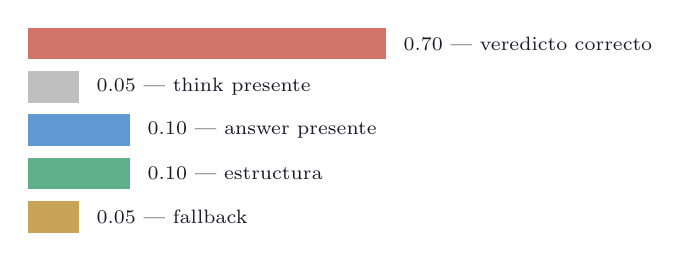
\begin{tikzpicture}[every node/.style={font=\scriptsize}]
        \fill[AccentRed!70]   (0,0.00) rectangle (4.55,0.40);
        \node[anchor=west, text=TextDark] at (4.65,0.20) {0.70 — veredicto correcto};
        \fill[gray!50]        (0,-0.55) rectangle (0.65,-0.15);
        \node[anchor=west, text=TextDark] at (0.75,-0.35) {0.05 — think presente};
        \fill[AccentBlue!70]  (0,-1.10) rectangle (1.30,-0.70);
        \node[anchor=west, text=TextDark] at (1.40,-0.90) {0.10 — answer presente};
        \fill[AccentGreen!70] (0,-1.65) rectangle (1.30,-1.25);
        \node[anchor=west, text=TextDark] at (1.40,-1.45) {0.10 — estructura};
        \fill[AccentGold!70]  (0,-2.20) rectangle (0.65,-1.80);
        \node[anchor=west, text=TextDark] at (0.75,-2.00) {0.05 — fallback};
      \end{tikzpicture}
    \end{column}
    \hfill
    \begin{column}{0.44\textwidth}
      \vspace{4mm}
      \cy{Algoritmo GRPO:}
      \vspace{5mm}

      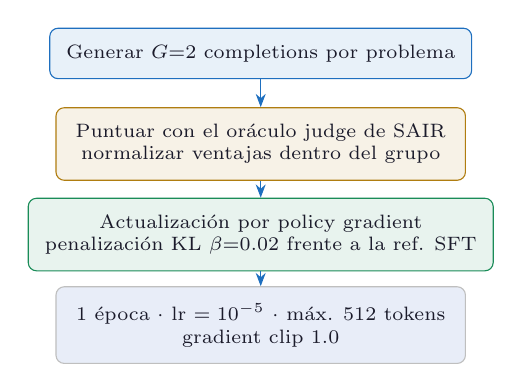
\begin{tikzpicture}[every node/.style={font=\scriptsize},
          ar/.style={-Stealth,thin,AccentBlue}]
        \node[draw=AccentBlue, fill=AccentBlue!10, rounded corners=3pt,
          minimum width=5.2cm, inner sep=6pt, align=center, text=TextDark]
        (g1) at (0,0) {Generar $G{=}2$ completions por problema};
        \node[draw=AccentGold, fill=AccentGold!10, rounded corners=3pt,
          minimum width=5.2cm, inner sep=6pt, align=center, text=TextDark]
        (g2) at (0,-1.15)
        {Puntuar con el oráculo judge de SAIR\\normalizar ventajas dentro del grupo};
        \node[draw=AccentGreen,fill=AccentGreen!10,rounded corners=3pt,
          minimum width=5.2cm, inner sep=6pt, align=center, text=TextDark]
        (g3) at (0,-2.30)
        {Actualización por policy gradient\\penalización KL $\beta{=}0.02$ frente a la ref. SFT};
        \node[draw=gray!50, fill=BoxBg, rounded corners=3pt,
          minimum width=5.2cm, inner sep=6pt, align=center, text=TextDark]
        (g4) at (0,-3.45)
        {1 época $\cdot$ lr $= 10^{-5}$ $\cdot$ máx. 512 tokens\\gradient clip 1.0};
        \draw[ar](g1)--(g2); \draw[ar](g2)--(g3); \draw[ar](g3)--(g4);
      \end{tikzpicture}
    \end{column}
  \end{columns}
\end{frame}

% ============================================================
% SLIDE 12  ·  CHEAT SHEET DISTILLATION
% ============================================================
\begin{frame}{Destilación de la Cheat Sheet}{Etapa 3: Compresión offline del conocimiento}
  \begin{columns}[T,onlytextwidth]
    \begin{column}{0.46\textwidth}
      \vspace{4mm}
      \cy{Pipeline:}
      \vspace{5mm}

      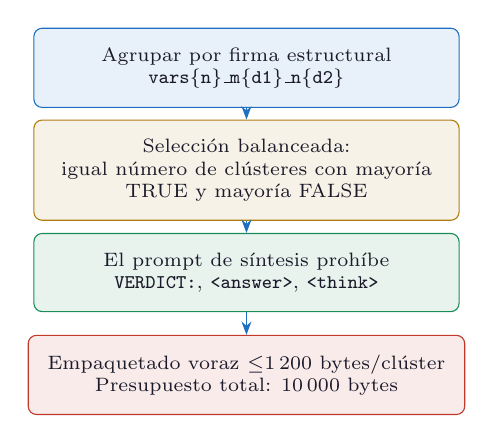
\begin{tikzpicture}[every node/.style={font=\scriptsize},
          ar/.style={-Stealth,thin,AccentBlue}]
        \node[draw=AccentBlue, fill=AccentBlue!10, rounded corners=3pt,
          minimum width=5.4cm, inner sep=7pt, align=center, text=TextDark]
        (s1) at (0,0)
        {Agrupar por firma estructural\\
          \texttt{vars\{n\}\_m\{d1\}\_n\{d2\}}};
        \node[draw=AccentGold, fill=AccentGold!10, rounded corners=3pt,
          minimum width=5.4cm, inner sep=7pt, align=center, text=TextDark]
        (s2) at (0,-1.3)
        {Selección balanceada:\\
          igual número de clústeres con mayoría \\ TRUE y mayoría FALSE};
        \node[draw=AccentGreen,fill=AccentGreen!10,rounded corners=3pt,
          minimum width=5.4cm, inner sep=7pt, align=center, text=TextDark]
        (s3) at (0,-2.6)
        {El prompt de síntesis prohíbe\\
          \texttt{VERDICT:}, \texttt{<answer>}, \texttt{<think>}};
        \node[draw=AccentRed,  fill=AccentRed!10,  rounded corners=3pt,
          minimum width=5.4cm, inner sep=7pt, align=center, text=TextDark]
        (s4) at (0,-3.9)
        {Empaquetado voraz $\leq$1\,200 bytes/clúster\\
          Presupuesto total: 10\,000 bytes};
        \draw[ar](s1)--(s2); \draw[ar](s2)--(s3); \draw[ar](s3)--(s4);
      \end{tikzpicture}
    \end{column}
    \hfill

    \begin{column}{0.50\textwidth}
      \vspace{3mm}
      \cy{Fallo de v1 y corrección en v2:}
      \vspace{4mm}

      \begin{alertblock}{v1: Colapsó hasta un 20\% de accuracy}
        Los clústeres dominados por FALSE filtraban tokens de veredicto
        en la síntesis $\Rightarrow$ sesgo sistemático hacia FALSE
      \end{alertblock}

      \vspace{1.5mm}

      \begin{exampleblock}{v2: Agrupamiento balanceado}
        Se fuerza el mismo número de clústeres TRUE/FALSE +
        un prompt de síntesis dedicado prohíbe tokens de veredicto
      \end{exampleblock}

      \vspace{3mm}
      \cy{Entrada de preámbulo (prioridad 999):}
      \vspace{2mm}

      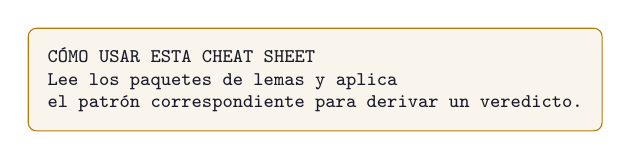
\begin{tikzpicture}
        \node[draw=AccentGold, fill=AccentGold!8, rounded corners=3pt,
          minimum width=6.0cm, inner sep=7pt,
          align=left, text=TextDark, font=\ttfamily\scriptsize]{%
          CÓMO USAR ESTA CHEAT SHEET\\
          Lee los paquetes de lemas y aplica\\
          el patrón correspondiente para derivar un veredicto.
        };
      \end{tikzpicture}
    \end{column}
  \end{columns}
\end{frame}

% ============================================================
% SLIDE 13  ·  DISTILL THEN DEPLOY
% ============================================================
\begin{frame}{Destilar y después desplegar}{Entrenamiento offline frente a evaluación online}
  \vspace{4mm}
  \centering
  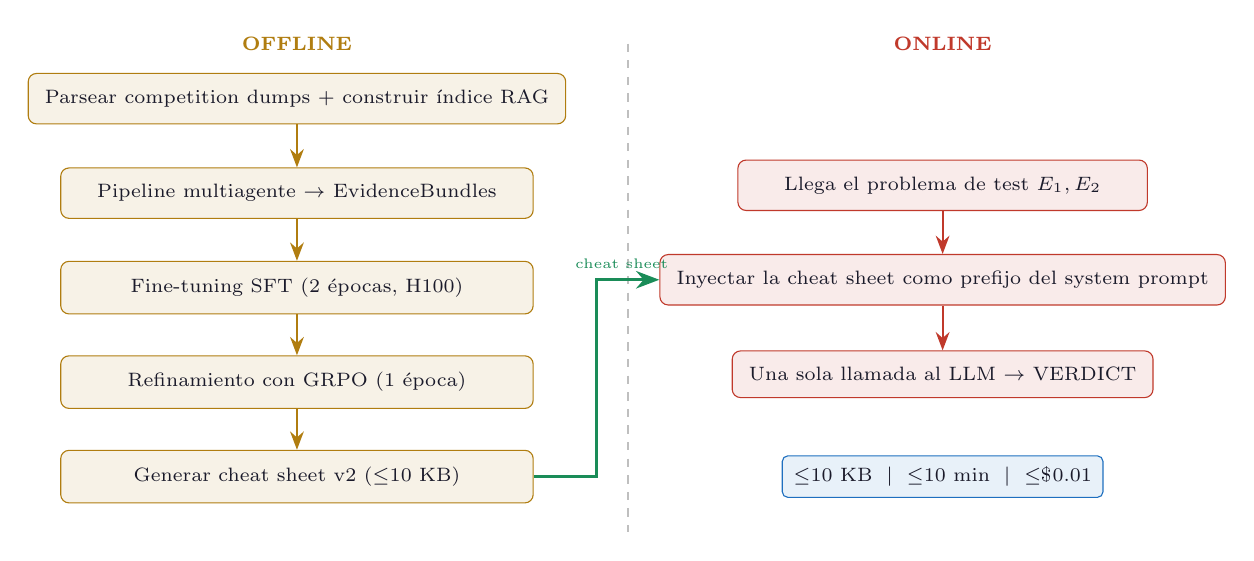
\begin{tikzpicture}[
      every node/.style={font=\scriptsize},
      OF/.style={draw=AccentGold,  fill=AccentGold!10,  rounded corners=3pt,
          minimum width=6.0cm, inner sep=6pt, align=center, text=TextDark},
      ON/.style={draw=AccentRed,   fill=AccentRed!10,   rounded corners=3pt,
          minimum width=5.2cm, inner sep=6pt, align=center, text=TextDark},
      ar/.style={-Stealth, thick},
    ]
    % OFFLINE
    \node[OF] (o1) at (-4.2, 2.0) {Parsear competition dumps + construir índice RAG};
    \node[OF] (o2) at (-4.2, 0.8) {Pipeline multiagente $\to$ EvidenceBundles};
    \node[OF] (o3) at (-4.2,-0.4) {Fine-tuning SFT (2 épocas, H100)};
    \node[OF] (o4) at (-4.2,-1.6) {Refinamiento con GRPO (1 época)};
    \node[OF] (o5) at (-4.2,-2.8) {Generar cheat sheet v2 ($\leq$10 KB)};
    \foreach \a/\b in {o1/o2,o2/o3,o3/o4,o4/o5}
    \draw[ar,AccentGold](\a)--(\b);

    % ONLINE
    \node[ON] (e1) at (4.0, 0.9) {Llega el problema de test $E_1, E_2$};
    \node[ON] (e2) at (4.0,-0.3) {Inyectar la cheat sheet como prefijo del system prompt};
    \node[ON] (e3) at (4.0,-1.5) {Una sola llamada al LLM $\to$ VERDICT};
    \foreach \a/\b in {e1/e2,e2/e3}
    \draw[ar,AccentRed](\a)--(\b);

    % Divider
    \draw[dashed,gray!50,thick](0,2.7)--(0,-3.5);
    \node[font=\scriptsize\bfseries, text=AccentGold] at (-4.2, 2.7) {OFFLINE};
    \node[font=\scriptsize\bfseries, text=AccentRed]  at ( 4.0, 2.7) {ONLINE};

    % Bridge
    \draw[ar,AccentGreen,very thick]
    (o5.east) -- ++(8mm,0) |- ([yshift=0mm]e2.west)
    node[pos=0.70, above, font=\tiny, text=AccentGreen]{cheat sheet};

    % Constraint badge
    \node[draw=AccentBlue, fill=AccentBlue!10, rounded corners=2pt,
      font=\scriptsize, text=TextDark, inner sep=4pt] at (4.0,-2.8)
    {$\leq$10 KB $\;|\;$ $\leq$10 min $\;|\;$ $\leq$\$0.01};
  \end{tikzpicture}
\end{frame}

% % ============================================================
% % SLIDE 14  ·  RESULTS
% % ============================================================
% \begin{frame}{Resultados experimentales}{Accuracy en distintas configuraciones de entrenamiento}
% \begin{columns}[T,onlytextwidth]
%   \begin{column}{0.46\textwidth}
%     \vspace{4mm}
%     \cy{Tabla de rendimiento:}
%     \vspace{3mm}

%     \setlength\arrayrulewidth{0.3pt}
%     \arrayrulecolor{gray!40}
%     \begin{tabular*}{\linewidth}{@{\extracolsep{\fill}}lcc}
%       \toprule
%       \rowcolor{BannerDark}
%       \textcolor{white}{\textbf{Configuración}} &
%       \textcolor{white}{\textbf{Acc.}} &
%       \textcolor{white}{\textbf{Parse}} \\
%       \midrule
%       \rowcolor{BoxBg}
%       Modelo base (sin fine-tuning)  & 0.50 & 0.75 \\
%       Solo agentes simbólicos        & 0.50 & ---  \\
%       \rowcolor{BoxBg}
%       Solo SFT (corpus de 20 problemas)   & 0.75 & 1.00 \\
%       SFT + GRPO (corpus de 20 problemas) & 0.75 & 1.00 \\
%       \rowcolor{AccentRed!15}
%       + cheat sheet \textbf{v1}
%         & \textcolor{AccentRed}{\textbf{0.20}} & 1.00 \\
%       \rowcolor{AccentGreen!15}
%       + cheat sheet \textbf{v2}
%         & \textcolor{AccentGreen}{\textbf{en progreso}} & 1.00 \\
%       \bottomrule
%     \end{tabular*}

%     \vspace{5mm}
%     \textcolor{gray}{\scriptsize
%       Infraestructura de entrenamiento: clúster DGX ($8\times$ NVIDIA H100)}
%   \end{column}
%   \hspace{0.03\textwidth}
%   \begin{column}{0.46\textwidth}
%     \vspace{4mm}
%     \begin{tikzpicture}
%       \node[draw=gray!50, dashed, fill=BoxBg,
%             rounded corners=4pt, minimum width=6.0cm, minimum height=6.0cm,
%             align=center, text=gray, font=\scriptsize]{%
%         \textbf{[IMAGE PLACEHOLDER]}\\[6pt]
%         Gráfico de barras de la progresión\\
%         de accuracy:\\[3pt]
%         Base $\to$ SFT $\to$ SFT+GRPO\\
%         $\to$ v1 (regresión) $\to$ v2\\[4pt]
%         Anotar la barra de v1 con\\
%         \textit{``sesgo hacia FALSE''}\\[4pt]
%         \textit{matplotlib, fondo claro}\\
%         \textit{barras AccentRed / AccentGreen}
%       };
%     \end{tikzpicture}
%   \end{column}
% \end{columns}
% \end{frame}


% ============================================================
% SLIDE 14  ·  RESULTS
% ============================================================
\begin{frame}{Resultados experimentales}{Accuracy en distintas configuraciones de entrenamiento}
  \begin{columns}[T,onlytextwidth]
    \begin{column}{0.46\textwidth}
      \vspace{4mm}
      \cy{Tabla de rendimiento:}
      \vspace{3mm}

      {\fontsize{6.5pt}{8pt}\selectfont
        \setlength\arrayrulewidth{0.3pt}
        \arrayrulecolor{gray!40}
        \begin{tabular*}{\linewidth}{@{\extracolsep{\fill}}lcc}
          \toprule
          \rowcolor{BannerDark}
          \textcolor{white}{\textbf{Configuración}} &
          \textcolor{white}{\textbf{Acc.}} &
          \textcolor{white}{\textbf{Parse}} \\
          \midrule
          \rowcolor{BoxBg}
          Modelo base (sin fine-tuning)  & 0.50 & 0.75 \\
          Solo agentes simbólicos        & 0.50 & ---  \\
          \rowcolor{BoxBg}
          Solo SFT (corpus de 20 problemas)   & 0.75 & 1.00 \\
          SFT + GRPO (corpus de 20 problemas) & 0.75 & 1.00 \\
          \rowcolor{AccentRed!15}
          + cheat sheet \textbf{v1}
          & \textcolor{AccentRed}{\textbf{0.20}} & 1.00 \\
          \rowcolor{AccentGreen!15}
          + cheat sheet \textbf{v2}
          & \textcolor{AccentGreen}{\textbf{en progreso}} & 1.00 \\
          \bottomrule
        \end{tabular*}
      }

      \vspace{5mm}
      \textcolor{gray}{\scriptsize
        Infraestructura de entrenamiento: clúster DGX ($8\times$ NVIDIA H100)}
    \end{column}
    \hspace{0.03\textwidth}
    \begin{column}{0.46\textwidth}
      \vspace{4mm}
      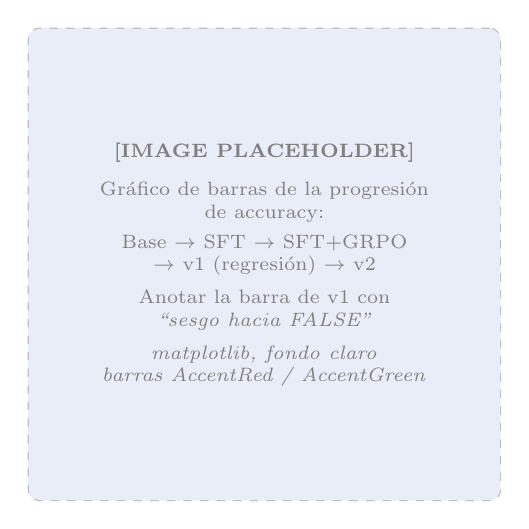
\begin{tikzpicture}
        \node[draw=gray!50, dashed, fill=BoxBg,
          rounded corners=4pt, minimum width=6.0cm, minimum height=6.0cm,
          align=center, text=gray, font=\scriptsize]{%
          \textbf{[IMAGE PLACEHOLDER]}\\[6pt]
          Gráfico de barras de la progresión\\
          de accuracy:\\[3pt]
          Base $\to$ SFT $\to$ SFT+GRPO\\
          $\to$ v1 (regresión) $\to$ v2\\[4pt]
          Anotar la barra de v1 con\\
          \textit{``sesgo hacia FALSE''}\\[4pt]
          \textit{matplotlib, fondo claro}\\
          \textit{barras AccentRed / AccentGreen}
        };
      \end{tikzpicture}
    \end{column}
  \end{columns}
\end{frame}


% ============================================================
% SLIDE 15  ·  CONCLUSIONS
% ============================================================
{
\setbeamertemplate{footline}{}
\begin{frame}[plain]
  \begin{tikzpicture}[remember picture,overlay]
    \fill[BannerDark] (current page.north west)
    rectangle ([yshift=-22mm]current page.north east);
    \node[font=\large\bfseries, text=white,
      anchor=north west, xshift=8mm, yshift=-5mm]
    at (current page.north west) {Conclusiones y trabajo futuro};
    \node[font=\scriptsize, text=AccentCyan,
      anchor=north west, xshift=8mm, yshift=-15mm]
    at (current page.north west) {ARD — Algebraic Reasoning Distiller};
    % footer bar
    \fill[BannerMid] (current page.south west)
    rectangle ([yshift=6mm]current page.south east);
    \node[font=\tiny, text=gray,
      anchor=south, yshift=1.5mm] at (current page.south)
    {Joaquín Mir Macías $\cdot$ José Andrés Ridruejo Tuñón $\cdot$
      Javier Ríos Montes $\cdot$ Miguel Montes Lorenzo $\cdot$
      Deep Generative Models $\cdot$ UPM 2025/2026};
  \end{tikzpicture}

  \vspace{20mm}
  \begin{columns}[T,onlytextwidth]
    \begin{column}{0.50\textwidth}
      \cy{Contribuciones clave:}
      \vspace{2mm}
      \begin{itemize}\setlength\itemsep{3pt}
        \item[\textcolor{AccentGreen}{$\checkmark$}]
              Pipeline multiagente: razonamiento \textbf{simbólico} + \textbf{neuronal}
        \item[\textcolor{AccentGreen}{$\checkmark$}]
              SFT $\to$ GRPO bajo \textbf{restricciones severas de recursos}
        \item[\textcolor{AccentGreen}{$\checkmark$}]
              Identificación y corrección del \textbf{sesgo de veredicto} de la cheat sheet (v1 $\to$ v2)
        \item[\textcolor{AccentGreen}{$\checkmark$}]
              Reproducible en DGX (Docker + \texttt{uv})
      \end{itemize}
      \vspace{3mm}
      \cy{Lecciones aprendidas:}\\[2pt]
      \scriptsize El \textbf{balanceo} de datos es crítico. El prompt de síntesis debe
      \textit{desacoplar} la generación del juicio.
      La degradación elegante permite un despliegue robusto.
    \end{column}
    \hfill
    \begin{column}{0.46\textwidth}
      \gd{Trabajo futuro:}
      \vspace{2mm}
      \begin{itemize}\setlength\itemsep{3pt}
        \item[\textcolor{AccentGold}{$\triangleright$}]
              Completar la cheat sheet \textbf{v2} sobre el corpus completo de 1\,761 problemas
        \item[\textcolor{AccentGold}{$\triangleright$}]
              Búsqueda \textbf{exhaustiva} de magmas de orden 4
        \item[\textcolor{AccentGold}{$\triangleright$}]
              Destilar en \textbf{modelos más pequeños} ($<$3B parámetros)
        \item[\textcolor{AccentGold}{$\triangleright$}]
              Refinamiento iterativo de la cheat sheet mediante un bucle GRPO
      \end{itemize}
      \vspace{3mm}
      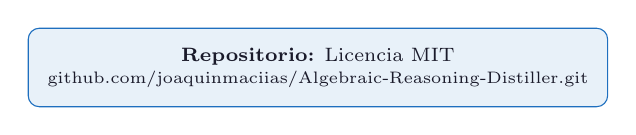
\begin{tikzpicture}
        \node[draw=AccentBlue, fill=AccentBlue!10, rounded corners=4pt,
        inner sep=7pt, align=center, text=TextDark, font=\scriptsize]{%
        \textbf{Repositorio:} Licencia MIT\\
        {\fontsize{6.5pt}{7.5pt}\selectfont
        github.com/joaquinmaciias/Algebraic-Reasoning-Distiller.git}
        };
      \end{tikzpicture}
    \end{column}
  \end{columns}
\end{frame}
}

\end{document}